\chapter{Existing technologies}

At the begining, I will introduce an existing solution of how to run PHP in a browser. 
The project \cite{Pib} aims to using compiled php interpreter into WebAssembly which allows to evaluate a PHP code.
The page has to import a specialized module php-wasm. 
A PHP code is evaluated by writing a specialized script block or manually by JavaScript and API.
PHP can afterwards interact with JavaScript using a specialized API.
At the first glance, that might be good enough solution, but they are several parts which can be problematic due to PHP semantics.
The solution doesn't solving globals. 
This is resonable, because this is server's job, but you are not able to get information about a query part or handling forms without writing a JavaScript code.
Next problem is a navigating. How a script can navigate to another script without an additional support code which has to be JavaScript.
These problems can be solved by following technologies and their integration.

\section{WebAssembly}

\cite{WebAssembly} is a new code format which can be run in today's browsers. 
It has a compact byte format and it's performance is near to a native code. 
WebAssembly is designed to be a compiling target of popular low-level languages like C or C++ due to it's memory model. 
It should be able to support languages with carbage collector in the future. 
Advantage of this format is a similarity with Javascript modules ES2015 after compilation into a machine code. 
This enables browsers to execute it by a JavaScript runtime. 
So it's security is as good as a code written in Javascript. 
Because of the same runtime, WebAssembly can call Javascript and vice versa.

Despite of supporting to run WebAssembly in browser, the browser can't load it as a normal ES2015 module yet.
WebAssembly Javasrcipt API was created in order to be able to load a WebAssembly to browser using JavaScript.

\section{Mono}

Mono is a .NET runtime which aims to mobile platforms. 
Recently, they started to support \cite{compilation} into WebAssembly.
This support allows executing CIL inside browsers.
The compilation has two modes.
The first one is compilation Mono runtime with all using assemlies.
The second only compiles Mono runtime which then can executes .dll files without further compilation of them into WebAssembly.
A consequence of these compilation into WebAssembly is enabling to call Javascript and WebAPI from .NET.

\section{Blazor}

Blazor is a framework which provides a convinient way how to write dynamic web pages using CSharp.
Blazor platform is devided into two \cite{Hosting_models} which have different approach how to create web applications. 
The first one is refered as Blazor Server App and has a similar methology like a common website written in PHP.
The interesting inovation using SignalR which is a comunication protocol between the server and a client.
But this thesis uses the second model which Microsoft refers as Blazor WebAssembly App enabling an offline support after loading the app into a browser.

\subsection{Blazor WebAssembly App}
From now on i will use Blazor App to refer Blazor WebAssembly App.
Blazor App can be devided into two parts.
The first part serves the main WebAssembly application and its additional resources which can be requested during a runtime.
The second part is WebAssembly wrapped together with an additional user code.
The division enables to choose a place for implementation of bussiness logic.
If there is a bad connection, we can move the mejority of bussiness logic to client and use the server for connection to a database, otherwise we can use client only for rendering the page. It consists of the following components. 
Kestrel with ASP.NET libraries provide server part of application.
Mono runtime compiled to WebAssembly runs CSharp code inside browser.
WebAssembly is important for be able to interact with DOM and JavaScript using CSharp without additional plugin which was necessary for older technologies like Microsoft Silverlight.
Blazor's libraries provides constructs for manipulation with DOM and WebAPI together with rendering the page and JavaScript interop.
And there are user code which using the libraries for creating dynamic pages with CSharp.
A better imagination, how the app is situated on client side, can be represented by  the figure \ref{img01:wasm} copied from \cite{Glick2018}.

\begin{figure}[H]\centering
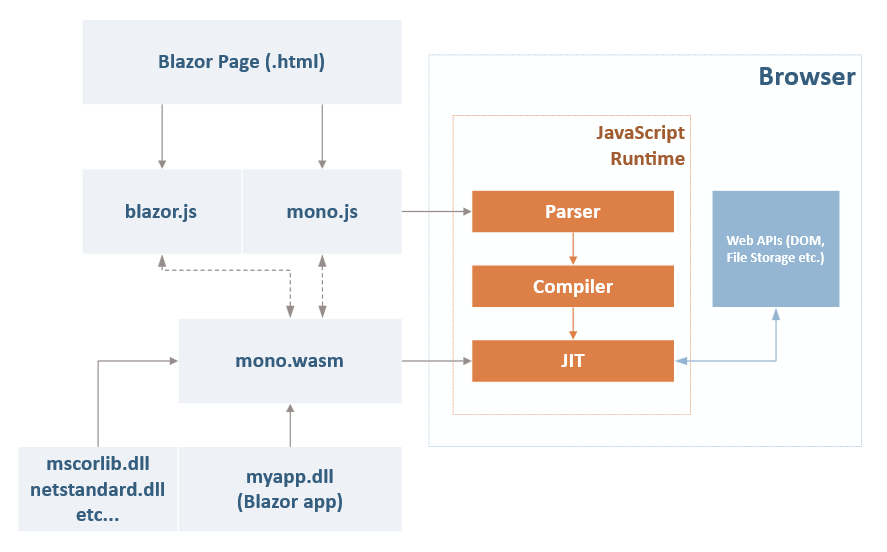
\includegraphics[width=140mm, height=100mm]{./img/BlazorExecution}
\caption{Running a Blazor WebAssembly App on client-side.}
\label{img01:wasm}
\end{figure}

Technical details of interop with a browser is one part of the Blazor App.
The main part is an architecture of the libraries.
A common approach how to create a page is using the markup language Razor.
There already exists Razor in common ASP.NET website where .cshtml extensions consist of this markup.
Unfortunately the markup used in BlazorApp has the same name.
From now on i will use Razor for the markup language which is content of .razor files in Blazor App.
Because interleaving of HTML with other language turns out to be useful, the Razor uses spacial characters to identify CSharp code in HTML and convert it to rich content pages.
A significant purpose of Razor is for generating CSharp structures, which represents parts of page, during compilation time.
These structures have complex interface for rendering a page, so the markup is there in order to free user using complicated machanism for putting page together.

Blazor introduces Component which can represent a whole page or the part of it.
Components can be arbitrarily put together in order to form a desired page.
They can have different purposes, for example there is Router which takes care of routing the right page whenever the navigation is triggered.
Alongside components there is a dispatcher which suplies aditional services like logger to components when they are creating.
The last item, which isn' used transparently, is a WebAssemblyHost builder.
The builder configures the application and prepare the renderer which is used by components to render their content.

Balzor presents own virtual DOM to reduce changing a DOM directly in a browser in order to its demending performance.
\change[inline]{TODO: Render tree builder}
\change[inline]{TODO: Renderer}
\change[inline]{TODO: Diff algorithm}
\change[inline]{TODO: Page Update}
Rendering is based on the diff algorithm of Blazor.
When the page is rendered for the first time, the diff algorithm is not necessary and DOM is updated according to RenderBatch which is generated from RenderTreeBuilder.
After page update, the diff algorithm is executed before DOM update. This algorithm gereratech RenderBatch which only modifies elements, which was updated.

The algorithm uses sequence of numbers to identify which elements was modified.




The process of bootstrapping Blazor app to browser folows these steps. 
Server gets a request for Blazor app. 
The server responses with html page, which contains references to Javascript responsible to load the app. The Javascript code fetches remaing resources like .dll libraries and runs Mono module. 
The runtime initialise the application using user defined .dll libraries.

Remaing interaction is maintained by event handling.
I divides it into two type of actions.

The first type is a navigation.
The \cite{navigation} can be triggered by an anchor, form or filling up the address bar.
Address bar is handled seperated by browser.
The remainings ways is handled by Javascript.
Anchor is the one one which are is handled by Blazor app by default.
Javascript tries to invoke navigation handler in Blazor app using a Mono WebAssembly gateway.
This handler can be modified by user, but a default behavoir is implemented by a specialized component Router.
The Router finds out all components, which implements an IComponent interface and tries to render the page according to path matching.
The navigation can be redirected to server.

The second type is events invoked by UI like onchange. These events are registred by RenderTreeBuilder with their callbacks. When the event is triggered, Javascript call right callback.

\section{PeachPie}

\change[inline]{TODO: What is PeachPie}
\change[inline]{TODO: Compiling PHP to .NET}

\section{PHP}

\change[inline]{TODO: Classic web page in php}
